\documentclass[11pt,oneside,a4paper]{article}
\usepackage{hyperref}
\usepackage{graphicx}
\usepackage{float}

\title{Holonym: A Decentralized Identity Bridge for the Internet}
\author{Nanak Nihal Khalsa \\ \href{mailto:nanak@opsci.io}{nanak@opsci.io} 
    \and Caleb Tuttle \\ \href{mailto:caleb@opscientia.com}{caleb@opscientia.com}
	\and Lily Hansen-Gillis \\ \href{mailto:lily@labdao.com}{lily@labdao.com}
	\and Kushal Kahar \\ \href{mailto:kushal@opsci.io}{kushal@opsci.io}
    \and Shady El Damaty \\ \href{mailto:shady@opsci.io}{shady@opscientia.com}}

\begin{document}
\maketitle
%%%%%%%%%%%%%%%%%%%%%%%%%%%%
%%%%%% INTRODUCTION %%%%%%%
%%%%%%%%%%%%%%%%%%%%%%%%%%%%
\section*{Introduction}
	 \paragraph{Holo+Nym} Holonym is an identity protocol for smart contracts that uniquely bridges any web account with decentralized blockchain applications (dApps), putting the user in control of the persona they curate online. This idea was inspired by Nick Szabo, the first to introduce smart contracts and virtual personae in the late 90s [ref]. A Holo is defined as a whole greater than the sum of its parts, where each linked \textit{nym} provides a distinct bit of information about a person. In other words, Holos are on-chain records that link \textit{nyms} to create a user-owned and verified pseudonymous identity.  Holonym increases security for dApps through built-in sybil resistance, and decreases the risk of lost accounts through non-custodial wallet recovery. With Holonym, smart-contract computable identities are now available and empower vast new use-cases from trust-less marketplaces, off/on-chain reputation metrics, and token gated web applications. Holonym was built to increase the cost of Sybil attacks, intellectual property theft, and lost-wallets, a significant \$10b+ problem for "permission-less" blockchain applications that do not have a centralized authority to administer and verify claims by anonymous users \cite{opensea_tweet, dune_anal}.  
%%%%%%%%%%%%%%%%%%%%%%%%%%%%	
	\paragraph{Innovating Beyond OAuth} Under-the-hood of Holonym is an elegant solution that bridges OAuth, the defacto standard for identity verification on the internet, with user accounts secured by asymmetric encryption key pairs that allow users to read, write, and interact with dApps. In general, Holonym ports JSON web tokens (JWTs) and other cryptographically signed data from any web site or service and makes it available for blockchain applications. A guiding principle for Holonym is bringing existing web services together with emerging blockchain ecosystems that empower  community-owned digital spaces and economies through interoperable design patterns, self-custody of cryptographic identity, and flexible privacy preferences for how users interact on the web.
%%%%%%%%%%%%%%%%%%%%%%%%%%%%
	\paragraph{An Autonomous Identity Protocol} Holonym is a decentralized protocol, meaning that it is non-proprietary, and runs on a global network of nodes. The code is open source and available for anyone to implement, integrate, or fork into their own application. Holos are self-sovereign, meaning that they are controlled by the identity’s owner. Each Holo can only be created or modified by the entity that owns the cryptographic keys used to sign and authorize actions on the decentralized networks that the protocol is deployed on.
	
	Holonym is a low-level persistent identity layer for the internet that enables a variety of use cases, specifically for decentralized Apps (dApps) that require access to verified user metadata. Any dApp can access a publicly listed Holo, filter by, or compute on, associated data and resolve the results on the front-end of any arbitrary website. In other words, developers have incredible flexibility to write versatile “view functions” on the underlying Holonym database.
	
	\paragraph{dApps: Unstoppable Applications} dApps are web applications that execute their instructions, or smart contracts, on a distributed network of nodes that ensure tamper-free consensus and no single point of failure. Consensus is typically implemented on a blockchain, where the previous history of all dApps is public and permanently stored by the nodes in the network. dApps have the advantage over centralized web services in that they are interoperable and autonomous; this means their activity is completely transparent, under no central control, permanently recorded, can’t crash, be turned off, or shut down.


	
\section*{On-Chain Verifiable Credentials}	
Verifiable Credentials (VCs) are a digital schema for user-owned proofs and claims on identity that have seen challenges for adoption. A standard for VCs has emerged through the World Wide Web Consortium (W3C) in response to calls by regulators seeking to curb the monopolization of user data by big tech companies \cite{w3c}. 

[insert figure or graphic here depicting VC and how Holo improves on it]

A key drawback of the W3C VC schema is the reliance on off-chain data, introducing needless centralization or increased complexity through specialized dedicated networks like Ceramic.  

Holonym . They need not be verified off-chain like in W3C specifications; their existence on-chain is proof that they are verified. Holos reduce the verification's burden for both the verifier and the verified. This allows easier adoption from both users and dApps by substantially lowering the amount of time and money required to verify credentials.  We see a future in which Holos are used to get Web2 data on blockchain, much like oracle networks but better, whereas VCs are used as a self-sovereign ID across Web2 websites as use-cases. It is important to note that VCs can include links to Holos and vice versa; the two are complementary.

\section*{Existing Approaches to Identity}
Multiple approaches for identity and trust in Web3 exist with unique capabilities and shortcomings. Some with radically different approaches include:
	\begin{itemize}
		\item Verifiable Credentials, e.g. Ceramic and Disco
		\item Social attestation networks, e.g. Proof of Humanity \& BrightID
		\item On-chain resume / badge services, e.g. Rabbit Hole \& Project Galaxy
		\item Centralized federated identity, e.g. Magic Link \& traditional SSO
		\item Enterprise DID and SSI services, e.g. Evernym, BloomID, \& Mattr 
		\item Traditional KYC services, e.g. Blockpass \& Stripe
		
	\end{itemize}
	
	\textit{Verifiable Credentials } allows for scalable databases well-suited for storing identities. Ceramic supports verifiable credentials, but its method of verifiable credentials puts burden on the users and the verifiers; users must submit a proof of Twitter by tweeting their public key and proof of GitHub by posting a gist with their public key. Keybase has the same mechanism for verifying credentials. In fact, W3C specification for DIDs is meant to be flexible, which means that proofs can take any form. The downside of this is that it places a tremendous burden on the verifier if they want to verify multiple types of proofs: there is no unified interface for verifiable credentials. 
	Holonym provides a unified interface to verify any credential for both the user and the developer, which requires just a few clicks on the user's part and two lines of code on the developer's part. Holos are interoperable with W3C credentials.
	
	\textit{Social attestation networks such as Proof of Humanity and BrightID} provide a handful benefits such as a Universal Basic Income token and Sybil resistance. However, they are game-theoretically insecure and thus cannot be used for serious applications where bad actors can reap benefits (an attack can cost only \$10 \cite{ted}). They also require a significant amount of effort from both the users and verifiers, further preventing scaling. Although the protocols in their current form are not viable in the long-term, they were important steps to solve a critical problem.
	
	\textit{On-chain resume / badge services} provide pseudonymous credentials. They effectively show accomplishments but they are limited to skill- and experience-related uses, rather than security- and identity-related uses. They are interoperable with Holos as they can be linked to the same blockchain address which has a Holo.
	
	\textit{Centralized Federated Identity} achieves a unified, quasi-self-sovereign identity. Google SSOs are centralized and were not blockchain-compatible until being used with Web3Auth and the WTF protocol (both of which perform disparate tasks using Web2 SSOs). These have been well-adopted due to making verification for users and developers much easier, by bieng all through one centralized provider. However, the cenrtalized provider is a single-point of failure for applications. Holos provide  convenience to developers while remaining decentralized.
	
	\textit{Enterprise DID and SSI services} such as Evernym, BloomID, \& Mattr provide some benefits of DIDs for organizations. However, unlike Holonym, they do not address  the need for identity on decentralized blockchains. In fact, they are fundamentally incompatible with public blockchains without significant reliance on custom oracle solutions. They require a level of reliance on, and adoption of, their ecosystems, whereas Holonym is baked into public EVM blockchains, which enables composability with smart contracts and interoperability with dApps.
	
	\textit{Traditional KYC services} provide deep checks into not just identity but also legal status. Efforts are being made to put these on-chain. Holonym will be able to incorporate these KYC checks and legal name verifications from third-party protocols.
	
	\section*{Holonym: How it Works}
		Holonym works by forwarding web tokens to smart contracts which verify their data is truly signed by the OpenID provider, e.g. Google for a gmail account. Single sign-on (SSO) services (login with Google et al. buttons) return JSON web tokens (JWTs) with RSA or HMAC signatures. RSA signatures used by Google, Facebook, ORCID, and others have the benefit of being verifiable by anyone. ECDSA signatures could also work and be far easier to implement on EVM chains but unfortunately, few servers sign JWTs with Elliptic Curve signatures. 

		\begin{figure}[h!]
        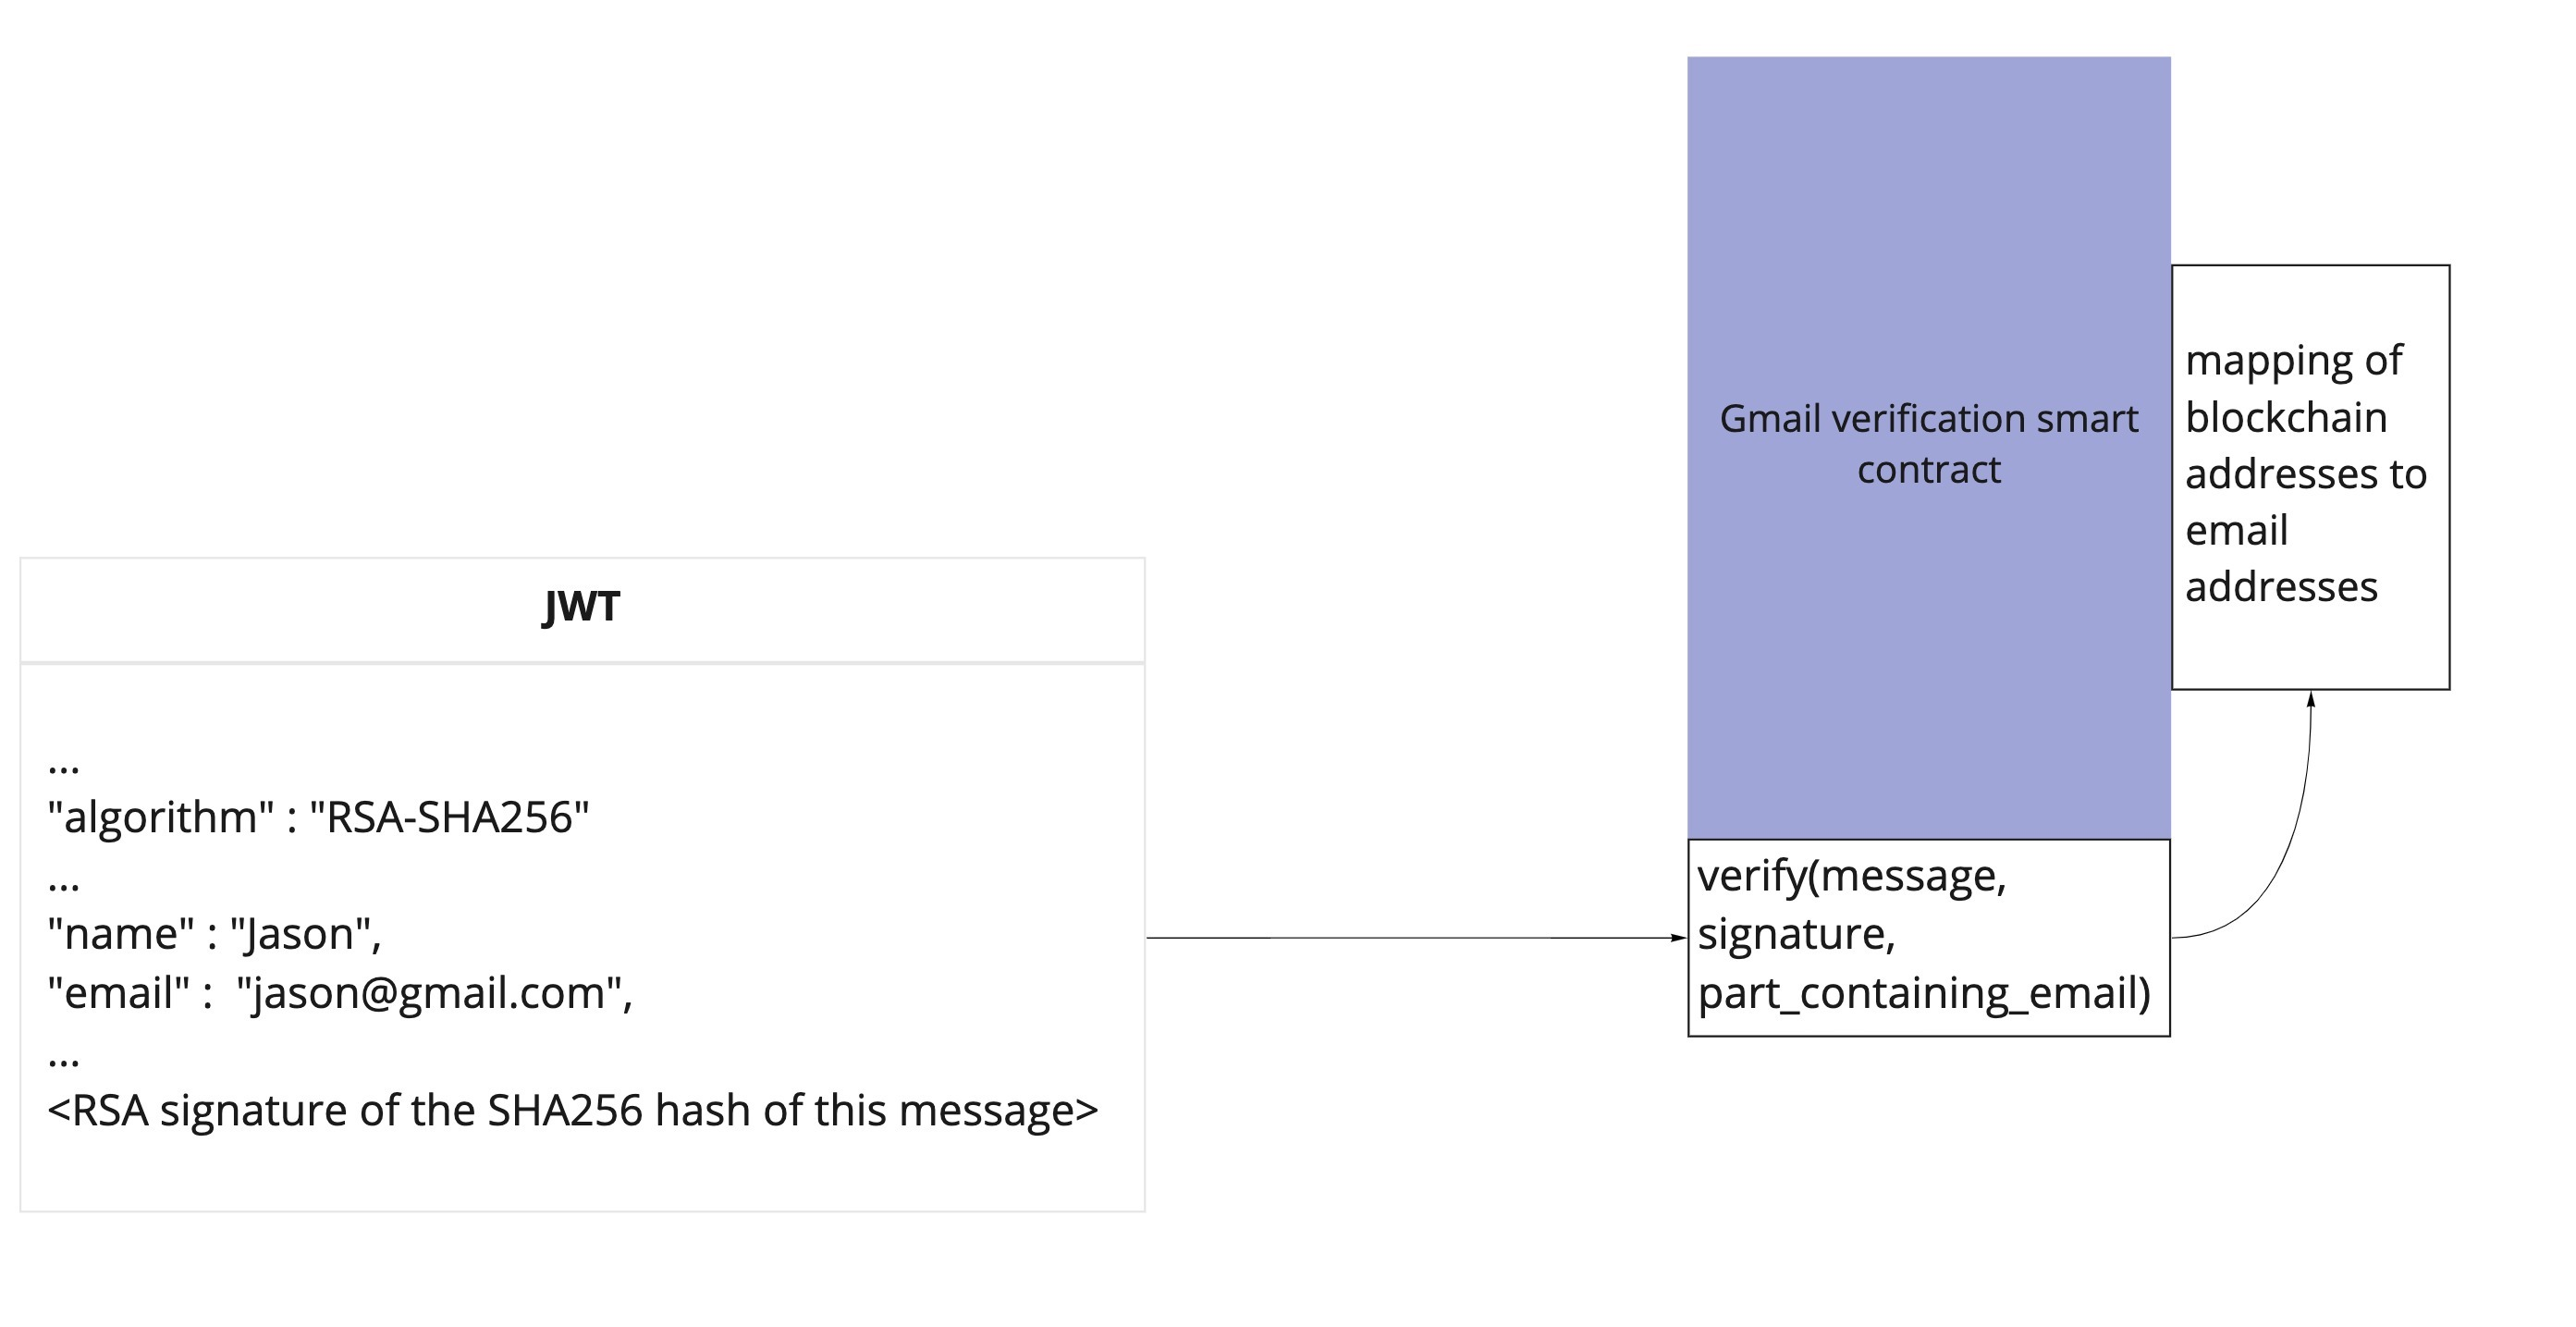
\includegraphics[width=\linewidth]{onChainJWT.jpeg}
        \caption{JWT verification process. The bidirectional mappings  allow O(1) lookups by credentials or blockchain addresses}
        \label{fig:jwtVerification}
        \end{figure}
		
		\pagebreak

		\subsection*{Asymmetric RSA Signatures}
		RSA Signatures are verified by sending the JWTs to the Verifier smart contracts, which use the 0x05 modular exponentiation precompile to compare the signature to a padded hash of the data which is signed (essentially, traditional RSA signature verification but on the EVM using the 0x05 precompile). For JWTs, the data to be hashed, padded, and signed is the readable aspect of the JWT, base64url encoded.
\\
\\
		\textbf{Verification of RSA signature}
		
		Below is the verification function for signature \textit{s}, public key \textit{(e,n)}, keccak256 hash function \textit{H}, and padding function \textit{P}. \textit{m} is the message, decoded from base64 format.
		\[ s^e (mod\ n)  == H(P((m))) \]
		
		Signature verification is similar to how all blockchain transactions work; transactions must be signed by the party transacting and verified by the blockchain. Here, instead of solely checking that a transaction is signed by the sender, the contract also checks the credentials are signed by Google, Facebook etc. 
		
	    \subsection*{Symmetric HMAC Signatures}
			HMAC signatures, such as those returned by Twitter, are not signed by an asymmetric key. They are not as straightforward to verify on-chain, since there is no public key anybody can use to verify a signature. Instead, the verifying key is identical to the signing key -- anyone who has the key can forge signatures! This is incompatible with public blockchains as bad actors can forge signatures with publicly known signing keys. Rather, symmetric keys are meant to be known only by the app (e.g., website with Twitter sign-in) and the provider (e.g. Twitter). 
			
		Holonym is working toward progressive decentralization of HMAC signatures. We are implementing zkSNARKs to prove a HMAC preimage without knowledge of the secret.  Meanwhile, we are running a centralized service which verifies an HMAC JWT and, upon success, makes a new JWT with an RSA signing key. On the roadmap to full decentralization, an intermediary step we may perform is verifying the JWT on a server with secure enclave, which eliminates most of the need for trust. zkSNARKs will eliminate all of Holonym's centralization.
			
		\subsection*{Prevention of Frontrunning}
			Once a blockchain-compatible  signature for credentials has been obtained, further steps are needed to proceed. The steps above by themselves would allow impersonation via frontrunning. Verifying a JWT on-chain leaves it in the mempool for anyone to steal and verify first by paying more gas. Thus, we employed a commit-reveal pattern for proving knowledge of a JWT amongst multiple blocks. This happens in the following three steps:
			\begin{enumerate}
				\item XOR hash of the JWT with owner's public key, and submit the hash of that result
				\item Wait for the current block to be finalized
				\item Submit the plaintext JWT for the smart contract to verify it.
			\end{enumerate}	  
			When 3. happens, the smart contract checks for a previous commitment; it XORs the hashed JWT with the sender's public key, then hashes the result. If a result exists and was submitted in an earlier block, it may check the result was not only known but also linked with the user's public key. In this block, the JWT remained unknown to all but the user because it was (XORed and) hashed before it was shared. After these steps confirm a JWT belongs to the submitter of the transaction, its signature can then be verified as mentioned previously. 
	\section*{Underlying Security of this Protocol}
		A few questions come up in the storing of JWTs on-chain. This is a protocol in alpha-stage dealing with an uncharted territory of on-chain verification of web2 credentials. We do not recommend storing credentials for any sensitive accounts on-chain until past the alpha version, despite having the protocol being informally reviewed by security experts.
		
		First is the question of whether users know blockchain data is public. We addressed this by clearly prompting users with the data that will be made public to ensure they consent to sharing it. We have thereby reduced the probability of user error to a negligible and tolerable amount.
		
		Second is the question of whether revealing OpenID tokens can allow for impersonation of the user. We have a uniquely identifiable ``aud" claim in the JWT so that no other website implementing OpenID will accept the tokens. Any secure website will reject JWTs submitted with ``aud" claim that restricts their audience to the Holonym protocol. Thus, revealed JWTs cannot be used to login to other websites that check JWTs. The only exceptions are atrociously insecure websites -- no serious institution would allow these tokens. An analogy would be a bar that accepts a Legoland Driver's license as a form of ID. Any service implementing the OpenID protocol only allows JWTs made for itself, not for Legoland. 		
	\section*{Future Steps}
	
	Holonym will enable far more than just on-chain ID, because on-chain ID enables so much more. It enables antisocial wallet recovery via the Lit Protocol. Currently, social recovery mechanisms rely on trusting others to help recover lost funds. Holos enable antisocial recovery, where one simply has to prove access to their own accounts (much like in Web2). Yet it provides this security and convenience without custodial wallets. 
	

    zkSNARKs of HMAC signatures is also on our roadmap to enable full decentralization. Once this is done, we will "throw away" the key so not even we can forge signatures. It will also pave the way to privacy-preserving proofs of identity on chain.
    
    We are also releasing a general-purpose "noracle" node package which can send generic web2 data to the blockchain using JSON. Currently, oracles are a relatively insecure and expensive middleman between a  website's data and the blockchain, which take all the money and give none to the website whose data is being monetized. While this was necessary for a while, Holo will enable a new phase of Oracles where participating websites will be paid for the tremendous value they are providing to the blockchain ecosystem. This will further secure blockchain and increase its data economy's efficiency.
	\section*{Use-Cases}	
	Holonym smart contracts enable accounts to be aggregated into a single Holo and indexed by the public cryptographic key of the owner. Public key lookup is a simple but powerful feature that allows the owner to link their interactions on a distributed network to “off-chain” and “offline” activity. Some examples of “view functions” that link a user’s data could include:

\paragraph{Discoverable Content by Verified Creators:} A bibliographic database of verified academic authors, where anyone can filter by field, institution, altmetrics, or perform regular expression search to find and directly request a paper from an author through a peer-to-peer routing protocol like IPFS.

\paragraph{Reputation Leaderboard:} A leaderboard directory of discoverable users ranked by reputation that have contributed to a Decentralized Autonomous Organization (DAO) by holding or staking governance tokens, participating in token-based voting, or executing smart contracts for DAO operations.

\paragraph{Token Gated Listings:} A listing board where members are only allowed to post if they have met some minimal deterministic criteria that can be executed by a smart contract and receive a token that makes them discoverable. For example, a medical imaging consultant that has passed training for administering a new device and received a Non Fungible Token (NFT) as a certificate proof of completion.

Many more possibilities abound, where a developer’s imagination is the only limitation.

	\section*{Conclusion}
		Holonym is a decentralized protocol that issues verfiable credentials via  on-chain verification of RSA and HMAC signatures. It can be used to increase blockchain adoption by preventing damage due to lost seed phrases. It can reduce plagiarism of creative content such as NFTs and any content in decentralized trust-based markets. From scientific journals to decentralized ebook, music or play-to-earn marketplaces, and even undercollateralized loans, Holo provides necessary blockchain infrastructure for trust. It even can be used to solve the oracle problem by establishing verified Web2 communications without trusting an oracle network. This opens up potential for blockchain-based data monetization for public data. While Holo's initial use case is decentralized science, all of these use cases start with verified on-chain identities, which Holo is the first to our knowledge to accomplish in a decentralized way.

\begin{thebibliography}{9}
	\bibitem{chainalysis} Chainalysis. (2022, February). \textit{The 2022 Crypto Crime Report}. Chainalysis. Retrieved March 27, 2022, from \url{https://go.chainalysis.com/rs/503-FAP-074/images/Crypto-Crime-Report-2022.pdf}
	
	\bibitem{chainlink} Elizabeth Licorish. (2021, November). \textit{Chainlink Announces Its Total Value Secured (TVS) Is Now Over \$75 Billion} Chainlink Today. Retrieved May 13, 2022, from \url{https://chainlinktoday.com/chainlink-announces-its-total-value-secured-tvs-is-now-over-75-billion/}
	
	\bibitem{dune_anal} @rchen8. (2022, March 27). Dune Analytics. \textit{OpenSea}. Retrieved March 27, 2022, from \url{https://dune.xyz/rchen8/opensea}
	
	\bibitem{opensea_tweet} OpenSea. (2022, January 27). \textit{OpenSea Tweet}. Twitter. Retrieved March 27, 2022, from \url{https://twitter.com/opensea/status/1486843201352716289}
	
	\bibitem{ted} @RoboTeddy. (2021, June). \textit{Proof of humanity: The cost of attack}. HackMD. Retrieved March 27, 2022, from  \url{https://hackmd.io/@RoboTeddy/SkFEYwptd}
	
    \bibitem{w3c} W3C. (2022, March). \textit{Verifiable Credentials Data Model v1.1
}. W3C. Retrieved May 13, 2022, from  \url{https://www.w3.org/TR/vc-data-model/}	

\end{thebibliography}
\end{document}